\documentclass[../main.tex]{subfiles}

\begin{document}

This chapter introduces the methods and techniques used in order to detect and measure cookie banners and the privacy options that they provide. Overall, the methodology of this project can be divided into 4 distinct steps. These steps are summarised, in chronological order, in the following list:

\begin{enumerate}
    \item \textbf{Dataset identification}: Collect a robust set of functioning websites to analyse and extract their cookie banners;
    
    \item \textbf{Data collection} Crawl the identified websites and effectively collect the relevant data such as the source code of the cookie notices as well as screenshots of the webpages;
    
    \item \textbf{Data sanitisation \& normalisation}: Sanitise and structure the collected data from the previous step is a searchable and user friendly data structure.
    
    \item \textbf{Data analysis}: Analyse and make sense of the collected cookie banners and their privacy options. 
\end{enumerate}

\section{Data Identification}
The first step is to identify websites that can be analysed further in the subsequent steps of this project. Using publicly available lists such as Tranco \cite{LePochat2019}, popular websites for the countries of interest were identified and used for further research. Identifying and utilising the most popular websites, from a wide range of categories, can show how the vast majority of users in a given country experience the web and can illustrate the impact of cookie banners and the privacy options that they offer.

Furthermore, country-specific lists, such as TopGR (\url{https://topgr.gr}), were also used to identify websites. This was done in order to handle local nuances that would otherwise be missed if this project used only Tranco for building its dataset. More specifically, country-specific lists aided the discovery of popular websites that do not use the Top Level Domain (TLD) of their country of origin. For instance, although British Airways (BA) is a UK company, they are using the \say{.com} TLD for their website and therefore, it would have been excluded from the dataset if the country-specific lists were not taken into account.

However, it is important to note that not all websites allow crawling and a lot of them explicitly state that they only allow \say{personal use} of their services and content to their visitors. In order to comply with the terms of use of the websites within the dataset, this project introduces two novel ways of respecting the restrictions imposed by the websites. These are summarised in the following list:

\begin{enumerate}
    \item A \say{robots exclusion standard} parser that verifies whether websites allow crawling by reading their robots.txt file;
    
    \item A \say{terms of service} (TOS) parser that makes best efforts to find exclusionary terms, such as \say{for personal use only}, in order to comply with the TOS of each website.
\end{enumerate}

\section{Data Collection}
The second step is to effectively identify and collect the cookie banners on the websites in the dataset. In order to do so, this project takes advantage of the \say{I don’t care about cookies} (IDCAC) list which provides an extensive selection of common CSS selectors that cookie banners use. More specifically, the CSS selectors from that list are parsed and then added to a database to be used by OpenWPM. Furthermore, an additional 64 selectors are added to the list which was identified during testing.

After the cookie selectors have been parsed and added to the database, OpenWPM uses them to identify the cookie banners within the dataset identified in the previous step. More specifically, OpenWPM has been extended by this project to detect the cookie notices within a given website. OpenWPM checks whether the visited website has any of the selectors from the IDCAC list and if so, the cookie notice’s HTML code, as well as its attributes, are added to a database for further analysis. Table \ref{tab:methods_openwpm_fields}, summarises the data that is being saved in the database after OpenWPM has successfully identified the cookie banner. 

\begin{table}[ht]
    \centering
    \begin{tabular}{@{}ll@{}}
    \toprule
        \textbf{Field} & \textbf{Description}                                   \\ \midrule
        HTML           & The full HTML code of the cookie banner.               \\
        size           & The width and height of the cookie banner.             \\
        position       & The x and y coordinates of the cookie banner in the    \\ 
                       & page.                                                  \\
        banner\_exists & Indicates whether the banner has been successfully     \\ 
                       & identified by OpenWPM.                                 \\
        selector       & The CSS selector that the cookie banner uses.          \\ \bottomrule
    \end{tabular}
    \caption{The cookie banner attributes that are saved in the database by OpenWPM.}
    \label{tab:methods_openwpm_fields}
\end{table}

\section{Data Sanitisation \& Normalisation}

After OpenWPM has completed crawling the websites in the dataset, the next step is to sanitize and normalize the collected data. To our knowledge, no standard exists for cookie banners and therefore, every website has a different implementation for their notices. Thus, the HTML code, as well as the options that they provide, can be drastically different from website to website. This can make data analysis extremely difficult since there is no clear or efficient way of querying arbitrary data and therefore, the data have to be transformed into a consistent data structure before processing it further. 

Firstly, the collected data have to be sanitised so that the privacy options that are offered by the cookie banners are identified and classified. In order to do so, the privacy options are categorised into 4 distinct categories. These are the affirmative, non-affirmative, informative and managerial categories and they are summarised in Table \ref{tab:privacy_options_categories}.

\begin{table}[ht]
    \centering
    \begin{tabular}{@{}ll@{}}
    \toprule
        \textbf{Category} & \textbf{Description}                                   \\ \midrule
        Affirmative       & Options that prompt users to accept the use of cookies \\
                          & such as \say{Accept all}.                                  \\
        Non-Affirmative   & Options that allow users to opt-out from cookie        \\ 
                          & tracking such as \say{Decline}.                            \\
        Informative       & Options that take users to informational pages such as \\
                          & the Privacy Policy page.                               \\
        Managerial        & Options that allow users to manage tracking options    \\ 
                          & and opt-out from certain trackers.                     \\ \bottomrule
    \end{tabular}
    \caption{The categories that the privacy options are classified into.}
    \label{tab:privacy_options_categories}
\end{table}

After the data have been sanitised they can be transformed into a consistent data structure that allows for efficient and easy analysis. More specifically, the arbitrary structure of the collected cookie notices is turned into formal SQL-like table format. This is done for the following reasons:

\begin{enumerate}
    \item \textbf{Accessibility}: Not everyone understands HTML and therefore, it might be hard for someone without programming skills to analyse the gathered data. Furthermore, not all websites use simple HTML for their cookie banners, like the one seen in Figure \ref{fig:methods_code}.
    
    \item \textbf{Efficiency}: Even experienced HTML developers might have a hard time analysing the thousands of cookie banners that were collected during this project.
    
    \item \textbf{Searchability}: Performing queries can be inefficient and inaccurate when having to search for this kind of data structure.
\end{enumerate}

For instance, Figure \ref{fig:methods_code}, depicts the HTML code from the HTML code of a cookie banner found in 9volto (www.9volto.gr) which contains a sentence informing users that the website uses cookies and an \say{Agree} button. After the sanitisation and normalisation steps, discussed in this section, the cookie banner is transformed into the data structure shown in Figure \ref{fig:methods_code_normalised}. Therefore, this can then be transferred to a MySQL table or an Excel sheet for efficient and easy analysis. The complete SQL-like data structure is summarised in Table \ref{tab:methods_normalised_schema}.

\begin{figure}[ht]
    \centering
    \begin{subfigure}[b]{0.49\textwidth}
        \centering
        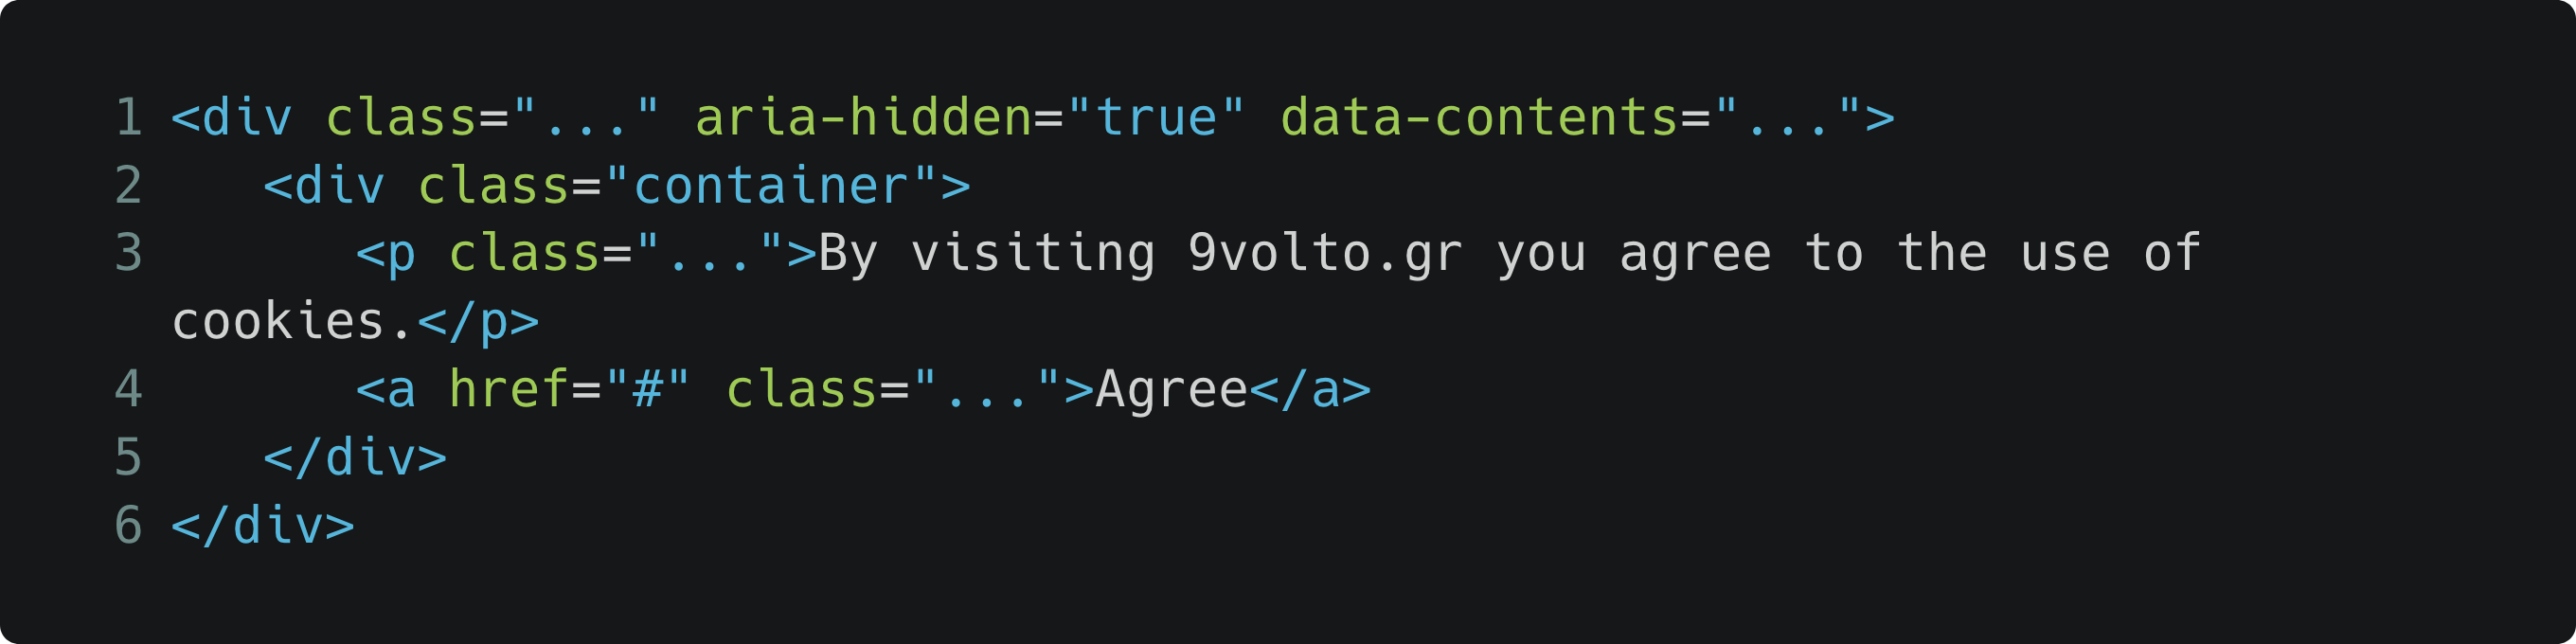
\includegraphics[width=\textwidth]{images/methodology/code.png}
        \caption{HTML code from 9volto.gr.}
        \label{fig:methods_code}
    \end{subfigure}
    \hfill
    \begin{subfigure}[b]{0.49\textwidth}
        \centering
        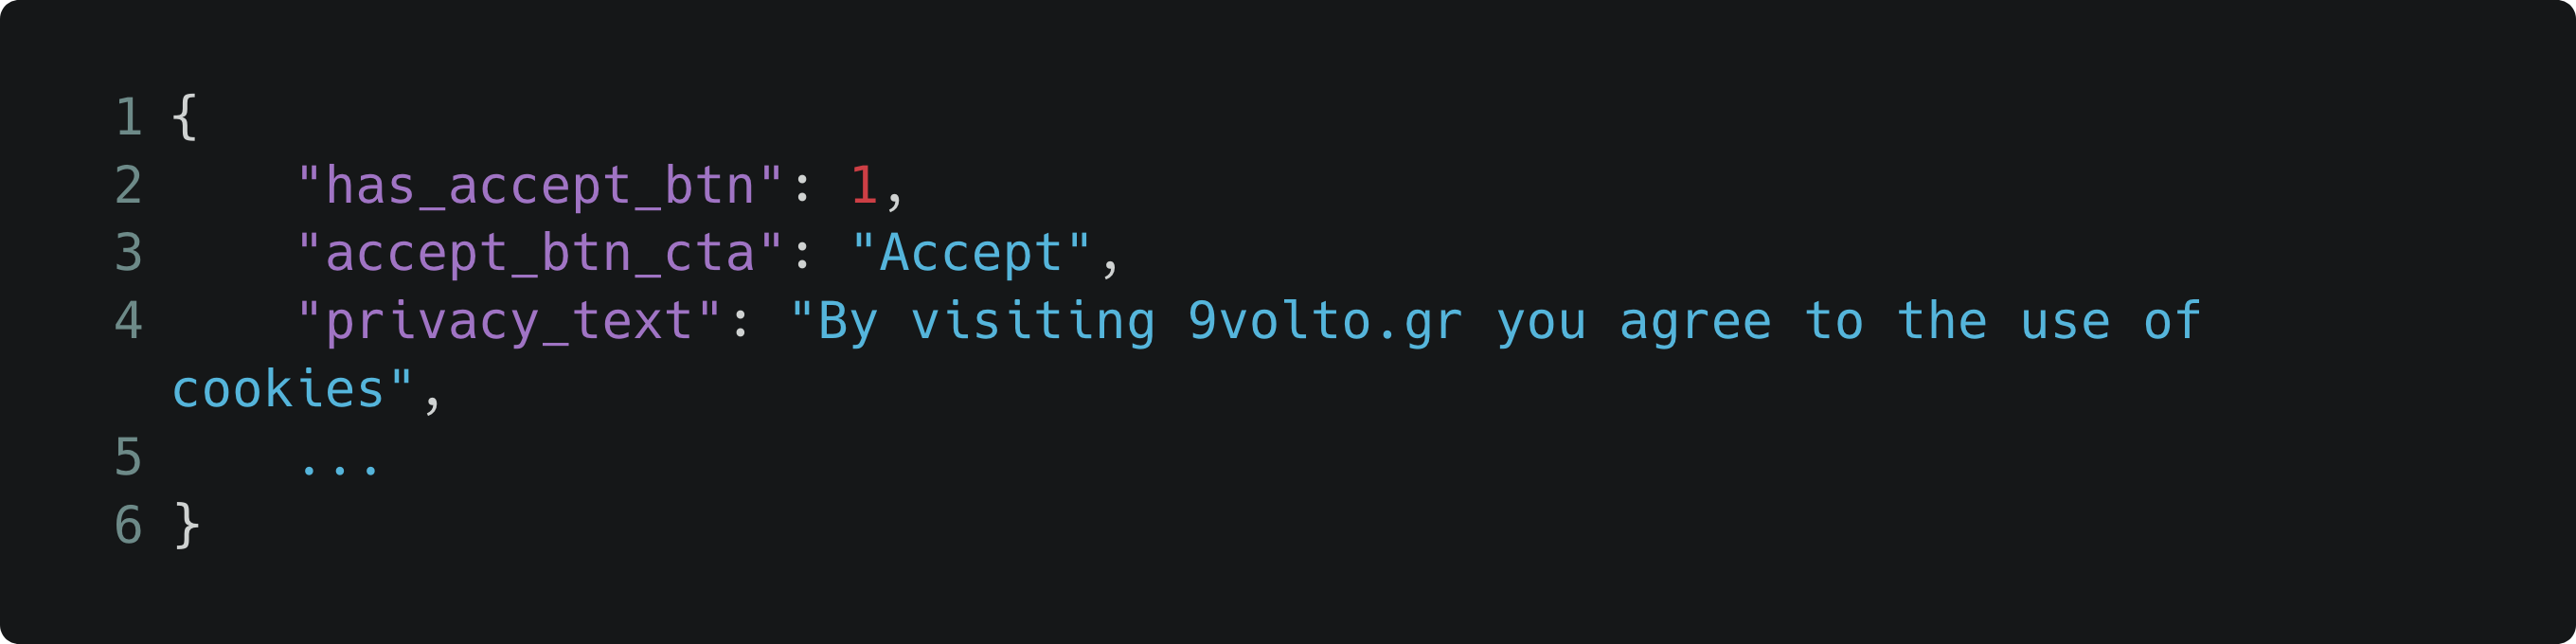
\includegraphics[width=\textwidth]{images/methodology/normalised.png}
        \caption{Normalised cookie banner.}
        \label{fig:methods_code_normalised}
    \end{subfigure}
    \caption{HTML code from a cookie banner before and after data sanitisation \& normalisation.}
    \label{fig:methods_html_code}
\end{figure}


\section{Data Analysis}
\label{sec:methodology_analysing_data}
After the data has been sanitised and normalised in a table-like data structure, the next step is to analyse the data in order to answer the research questions. While the data can be exported in a number of different applications, such as Microsoft’s Excel, this project retains the data in the database that was created in the previous steps in order to take advantage of SQL’s powerful and fast querying syntax and features. Where SQL fails to extract the required data, Python scripts have been used to perform more advanced analysis.
   
As before, the results are presented in a table-like format that can be converted into useful plots or exported in other applications for further analysis.

\section{Summary}
This chapter introduced the methods used and developed to detect cookie banners and analyse the privacy options that they give to users. In summary, this project’s methodology consists of 3 distinct steps. Firstly, popular websites from the target country are identified using open-source lists such as Tranco. Importantly, this project takes extra steps and makes best efforts to comply with each website's rules on crawling. Secondly, the cookie banners and their privacy options are identified and saved with the aid of OpenWPM as well as building on previous similar research to improve performance as well as retrieve more accurate data. The third step introduces a novel technique that structures the collected data in table format to allow for easy and efficient analysis. Finally, the structured data are analysed using SQL and Python in order to answer the research questions set by this project. Figure \ref{fig:methods_steps}, depicts the three methodology steps, as well as their sub-tasks, that were discussed in this chapter.

\begin{figure}[ht]
    \centering
    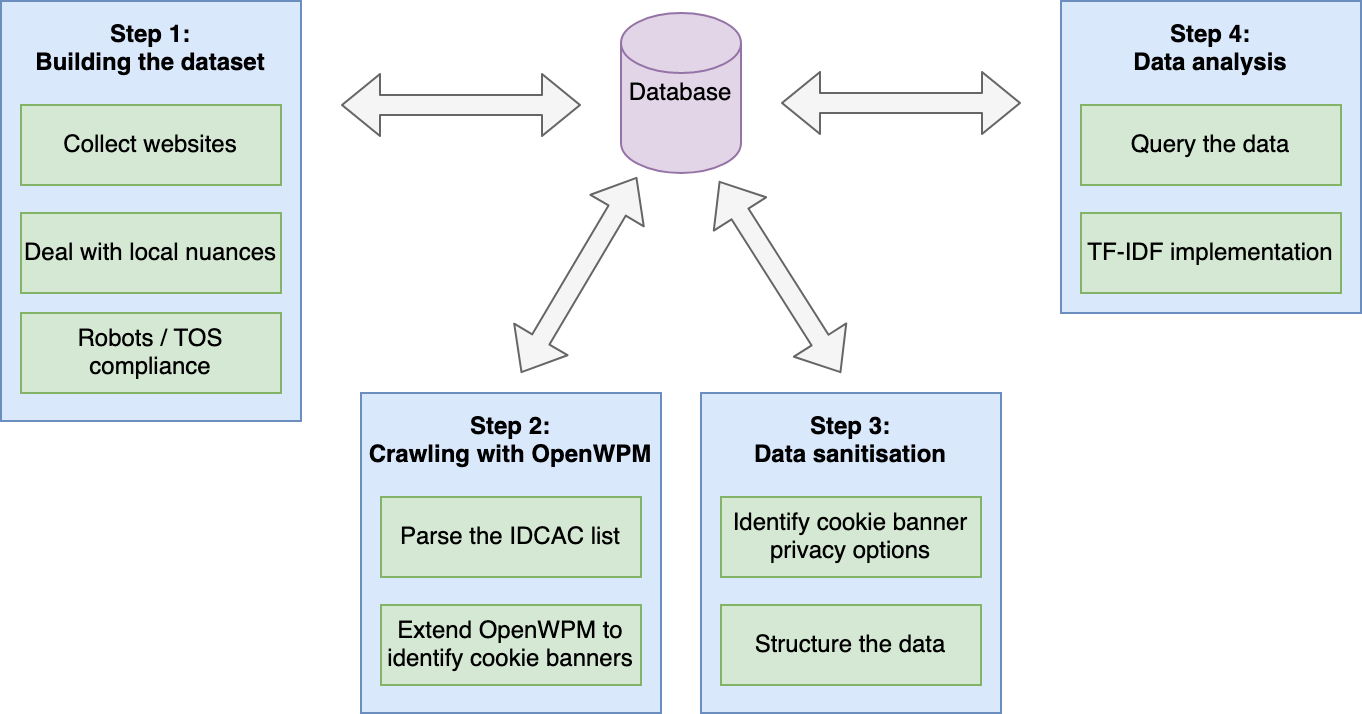
\includegraphics[width=\textwidth]{images/methodology/steps.png}
    \caption{The 4 steps of this project and their sub-tasks.}
    \label{fig:methods_steps}
\end{figure}

\end{document}